\documentclass[12pt]{article}
\usepackage{fix-cm}

\usepackage[paperwidth=48in, paperheight=36in, margin=0.6in, top=0.4in, bottom=0.4in]{geometry}
\usepackage[utf8]{inputenc}
\usepackage[T1]{fontenc}
\usepackage{lmodern}
\usepackage{graphicx}
\usepackage{booktabs}
\usepackage{amsmath, amssymb}
\usepackage{xcolor}
\usepackage{url}
\usepackage[numbers,sort&compress]{natbib}
\usepackage{multicol}
\usepackage{calc}
\usepackage{hyperref}
\hypersetup{colorlinks=true, linkcolor=navy, citecolor=indigo, urlcolor=indigo}

\pagestyle{empty}
\setlength{\parindent}{0pt}
\setlength{\parskip}{8pt}
\setlength{\columnsep}{0.45in}
\setlength{\columnseprule}{0.6pt}

% ── Colors ───────────────────────────────────────────────────────────────────
\definecolor{navy}{HTML}{1e3a5f}
\definecolor{indigo}{HTML}{6366f1}
\definecolor{panelbg}{HTML}{D8E0FF}
\definecolor{darktext}{HTML}{0f172a}
\definecolor{rose}{HTML}{f43f5e}
\definecolor{sectborder}{HTML}{205DA4}

\def\columnseprulecolor{\color{indigo!30}}

% ── Font sizes for poster ───────────────────────────────────────────────────
\newcommand{\posterbody}{\fontsize{26}{32}\selectfont}
\newcommand{\postersmall}{\fontsize{22}{27}\selectfont}
\newcommand{\posteritem}{\fontsize{24}{30}\selectfont}
\newcommand{\postersection}{\fontsize{34}{40}\selectfont}
\newcommand{\postersubsection}{\fontsize{28}{34}\selectfont}

% ── Section header box (styled like the posterdown examples) ─────────────────
\newcommand{\posterblock}[1]{%
  \vspace{10pt}%
  \noindent\colorbox{panelbg}{\parbox{\dimexpr\linewidth-2\fboxsep}{%
    \vspace{4pt}\centering\color{navy}\bfseries\postersection #1\vspace{4pt}}}%
  \vspace{6pt}\par%
}

% ── Highlight callout ────────────────────────────────────────────────────────
\newcommand{\highlightbox}[1]{%
  \noindent\fcolorbox{indigo}{panelbg}{\parbox{\dimexpr\linewidth-2\fboxsep-2\fboxrule}{%
    \centering #1}}%
}

% ══════════════════════════════════════════════════════════════════════════════
\begin{document}
\posterbody

% ══════════════════════════════════════════════════════════════════════════════
%  TITLE BOX — full-width colored banner
% ══════════════════════════════════════════════════════════════════════════════
\noindent\colorbox{panelbg}{\parbox{\dimexpr\textwidth-2\fboxsep}{%
  \vspace{16pt}
  \begin{minipage}[c]{3.6in}
    \centering
    
\includegraphics[width=3.2in]{figures/hdsi-blue-gold.png}
  \end{minipage}%
  \hfill
  \begin{minipage}[c]{\dimexpr\textwidth-8.8in-4\fboxsep}
    \centering
    {\fontsize{60}{68}\selectfont\bfseries\color{navy}
      Toward Accelerated LLM Inference:\\[8pt]
      Porting and Evaluating Diffusion-Based\\[4pt]
      Speculative Decoding on TPU\par}
    \vspace{14pt}
    {\fontsize{28}{34}\selectfont
      Aaron Feng\textsuperscript{1} \quad
      Zhongyan Luo\textsuperscript{1} \quad
      Son Nguyen\textsuperscript{1} \quad
      Andy Huang\textsuperscript{1} \quad
      Hao Zhang\textsuperscript{1}~(Mentor)\par}
    \vspace{8pt}
    {\fontsize{24}{30}\selectfont \textsuperscript{1}Halıcıoğlu Data Science Institute, UC San Diego\par}
  \end{minipage}%
  \hfill
  \begin{minipage}[c]{3.6in}
    \centering
    
\includegraphics[width=2.6in]{figures/qrcode.png}\\[6pt]
    {\fontsize{20}{24}\selectfont\bfseries\color{navy} Project Website}
  \end{minipage}
  \vspace{16pt}
}}

\vspace{0.15in}

% ══════════════════════════════════════════════════════════════════════════════
%  THREE-COLUMN BODY
% ══════════════════════════════════════════════════════════════════════════════
\begin{multicols}{3}
\color{darktext}
\posterbody

% ──────────────────────────────────────────────────────────────────────────────
%  LEFT COLUMN
% ──────────────────────────────────────────────────────────────────────────────

\posterblock{Problem \& Motivation}

\posteritem
\begin{itemize}\setlength\itemsep{6pt}
  \item LLM decoding is \textbf{inherently sequential}: generating $n$ tokens
        requires $n$ target-model forward passes---latency grows linearly.
  \item \textbf{Speculative decoding} uses a lightweight \emph{draft model} to
        propose candidates; the target verifies in one batched pass. Good drafts
        $\Rightarrow$ multiple tokens accepted per step.
  \item \textbf{Our contribution:} Port DFlash---a diffusion-based
        drafter---from GPU/PyTorch to TPU/JAX inside \texttt{tpu-inference}.
        Benchmark Qwen3-4B across 9 datasets.
  \item \textbf{Key TPU advantage:} Verification cost is \textbf{flat from
        $K$=16 to $K$=128} (only 0.97$\times$), while GPU scales to 2.3$\times$.
\end{itemize}

\posterblock{Background}

\posteritem
{\postersubsection\bfseries\color{navy} Speculative Decoding\par}\vspace{2pt}
\begin{itemize}\setlength\itemsep{4pt}
  \item Draft $n$ candidate tokens with a fast model, then verify all at once
        via rejection sampling.
  \item Key metric: $\tau$ = average accepted tokens per draft step.
\end{itemize}

\vspace{6pt}
{\postersubsection\bfseries\color{navy} Draft Model Approaches\par}\vspace{2pt}
\begin{itemize}\setlength\itemsep{4pt}
  \item \textbf{N-gram:} Fast but low $\tau$ (poor distribution approximation).
  \item \textbf{Eagle3:} Autoregressive drafter, $O(k)$ sequential forward passes.
  \item \textbf{DFlash:} Diffusion-based \emph{block drafter}---generates all
        16 tokens in \textbf{one forward pass} via non-causal attention.
        Draft cost is $O(1)$ regardless of block size.
\end{itemize}

\vspace{6pt}
{\postersubsection\bfseries\color{navy} DFlash Architecture\par}\vspace{2pt}
\begin{itemize}\setlength\itemsep{4pt}
  \item 4-layer transformer with \textbf{non-causal block attention}.
  \item Reuses target model's embedding layer and LM head.
  \item Conditioned on hidden states from layers [1, 9, 17, 25, 33],
        projected via FC + RMSNorm.
  \item Trained on only 289K samples; outperforms Eagle3 (1.4M samples).
\end{itemize}

\posterblock{Methods: GPU $\rightarrow$ TPU}

\posteritem
\begin{enumerate}\setlength\itemsep{6pt}
  \item \textbf{Dual KV cache:} Paged KV (PagedAttention) for target; static
        JAX KV with \texttt{dynamic\_update\_slice} for draft.
  \item \textbf{Non-causal attention:} Draft layers use TPU
        \texttt{flash\_attention} with \texttt{causal=False}.
  \item \textbf{Critical bug fix---sequence-length inflation:}
        Phantom tokens ($\sim$15/step) corrupted RoPE embeddings.
        Fixing this \emph{nearly doubled performance:}\\
        \hspace*{1em}$\tau$: 2.49 $\to$ 4.48 \quad
        Speedup: 1.30$\times$ $\to$ 2.31$\times$
  \item \textbf{Hidden-state extraction:} Layers [1,9,17,25,33]
        concatenated, projected via FC + RMSNorm.
  \item \textbf{Method registration:} New \texttt{"dflash"} branch in
        \texttt{tpu\_runner.py} with prewarm support.
\end{enumerate}
\vspace{4pt}
Zero new vLLM dependencies. Full DFlash contract preserved.

% ──────────────────────────────────────────────────────────────────────────────
%  CENTER COLUMN
% ──────────────────────────────────────────────────────────────────────────────

\posterblock{Results}

\highlightbox{%
  \vspace{8pt}
  {\fontsize{40}{46}\selectfont\bfseries\color{navy} 2.31$\times$}~~{\fontsize{22}{26}\selectfont vLLM pipeline} \hfill
  {\fontsize{40}{46}\selectfont\bfseries\color{navy} 3.01$\times$}~~{\fontsize{22}{26}\selectfont Standalone V5P} \hfill
  {\fontsize{40}{46}\selectfont\bfseries\color{navy} $\tau$ = 5.42}~~{\fontsize{22}{26}\selectfont Avg.\ accepted}
  \vspace{8pt}
}

\vspace{6pt}
\posteritem
\begin{itemize}\setlength\itemsep{4pt}
  \item Qwen3-4B + DFlash-b16 on \textbf{9 datasets}, TPU V5P (4 chips).
  \item Math: \textbf{3.72$\times$} ($\tau$=6.71) ~|~ Code: \textbf{2.77$\times$}
        ($\tau$=5.09) ~|~ Chat: \textbf{1.96$\times$} ($\tau$=3.37).
  \item Peak: Math500 at \textbf{4.93$\times$} ($\tau$=8.80), \emph{exceeding}
        the GPU paper result ($\tau$=7.84).
\end{itemize}

\vspace{4pt}
\begin{center}
  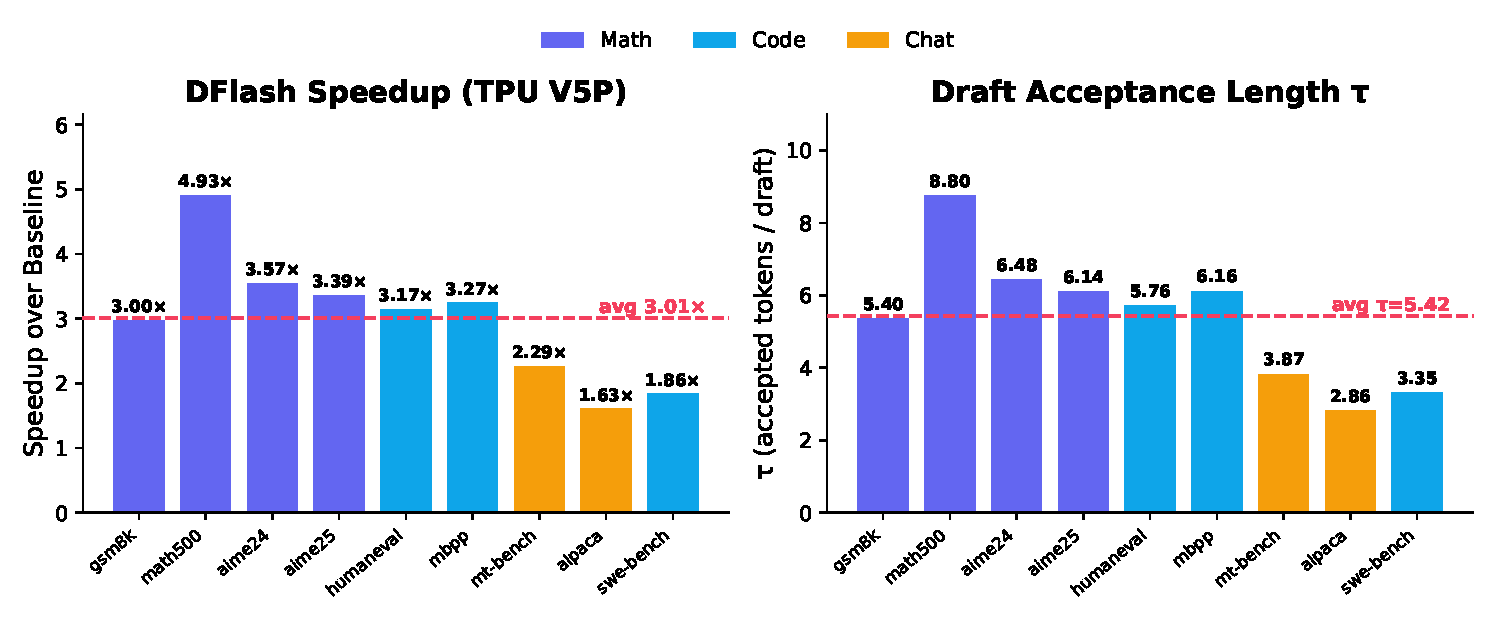
\includegraphics[width=\linewidth]{figures/summary_dashboard.pdf}
\end{center}

\posterblock{TPU vs GPU Draft Quality}

\begin{center}
  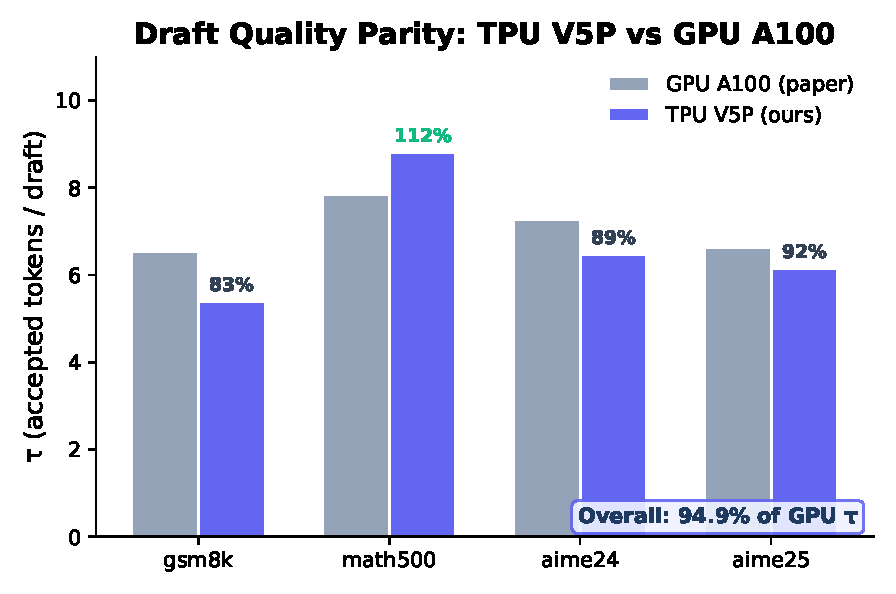
\includegraphics[width=0.95\linewidth]{figures/tpu_vs_gpu_parity.pdf}
\end{center}

\vspace{4pt}
\posteritem
\begin{itemize}\setlength\itemsep{4pt}
  \item \textbf{Draft quality parity:} TPU achieves 94.9\% of GPU $\tau$ overall.
  \item Math500 \emph{exceeds} GPU at 112\%---the only benchmark where TPU
        surpasses the original GPU implementation.
  \item Remaining $\sim$5\% gap attributed to bf16 precision and attention kernel
        differences.
\end{itemize}

% ──────────────────────────────────────────────────────────────────────────────
%  RIGHT COLUMN
% ──────────────────────────────────────────────────────────────────────────────

\posterblock{Acceptance Rate by Position}

\begin{center}
  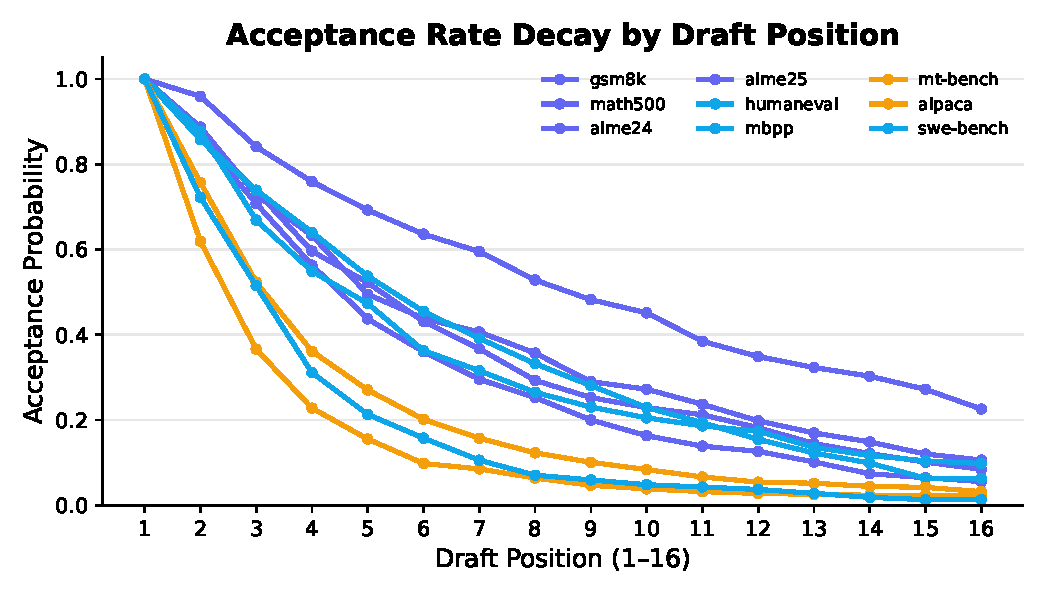
\includegraphics[width=\linewidth]{figures/acceptance_decay.pdf}
\end{center}

\vspace{2pt}
\posteritem
\begin{itemize}\setlength\itemsep{4pt}
  \item Math benchmarks maintain $>$70\% acceptance through position 8--10.
  \item Chat drops below 50\% by position 4--5 due to higher entropy.
  \item Non-causal attention allows position 16 to ``see'' all 15 neighbors
        bidirectionally, preserving quality at later positions.
\end{itemize}

\posterblock{Conclusion \& Future Work}

\begin{minipage}[t]{0.48\linewidth}
  \centering
  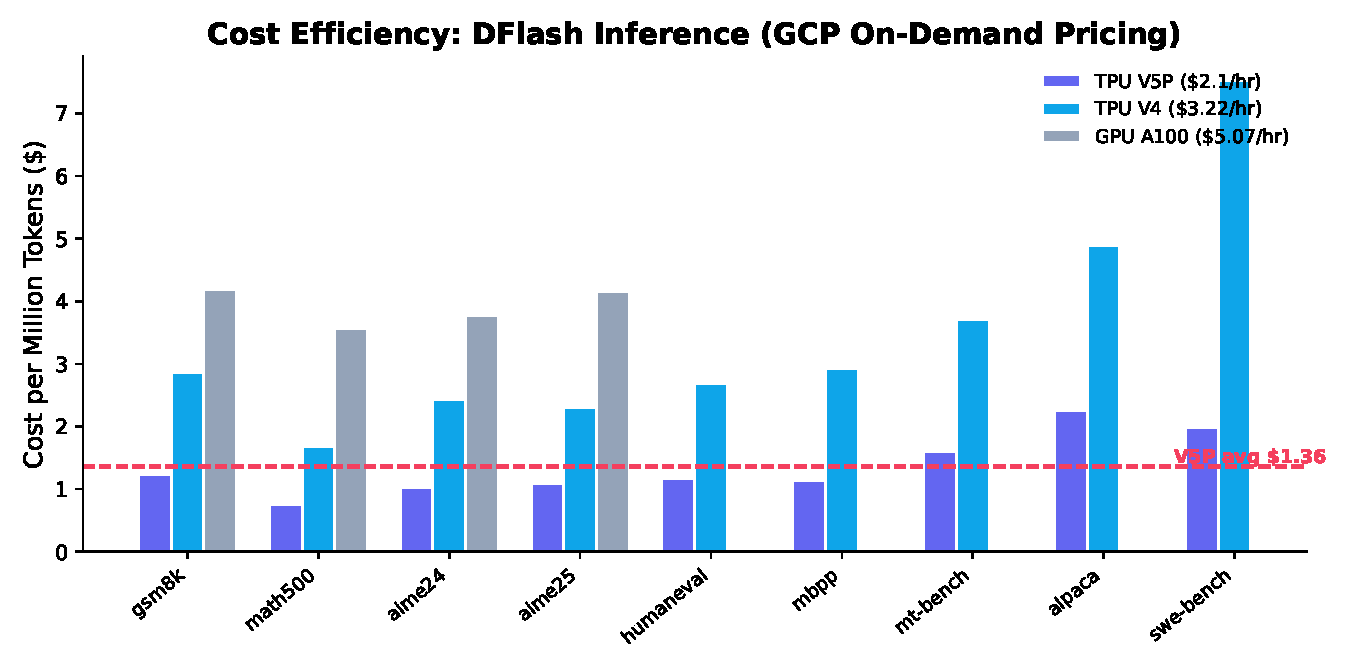
\includegraphics[width=\linewidth]{figures/cost_efficiency.pdf}
\end{minipage}\hfill
\begin{minipage}[t]{0.48\linewidth}
  \centering
  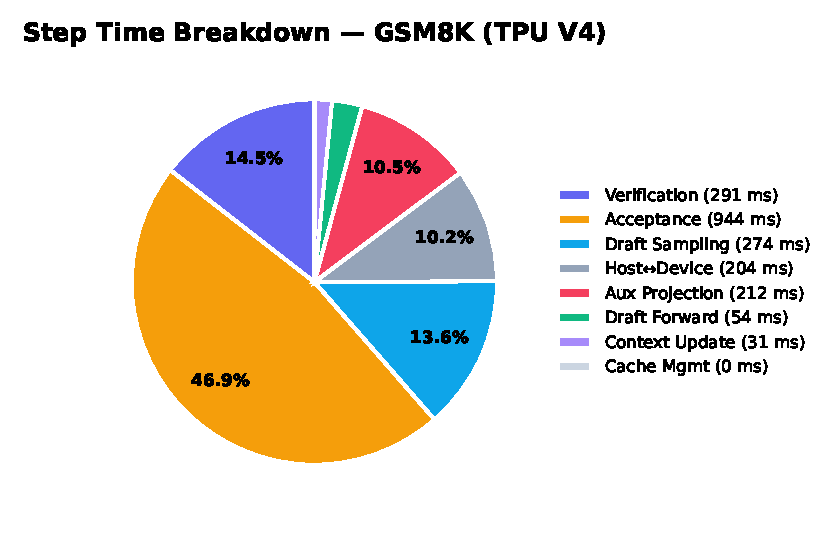
\includegraphics[width=\linewidth]{figures/profiling.pdf}
\end{minipage}

\vspace{8pt}
\posteritem
\begin{itemize}\setlength\itemsep{4pt}
  \item DFlash on TPU V5P: \textbf{3.01$\times$} standalone, \textbf{2.31$\times$}
        end-to-end pipeline speedup.
  \item Output quality is preserved---divergence is numerical (bf16), not errors.
  \item Pipeline overhead, not model compute, is the remaining bottleneck.
  \item TPU V5P + DFlash is the \textbf{most cost-efficient} option
        at \$1.36/M tokens average.
\end{itemize}

\vspace{4pt}
{\postersubsection\bfseries\color{navy} Future Work\par}\vspace{2pt}
\posteritem
\begin{itemize}\setlength\itemsep{4pt}
  \item \textbf{Wider blocks ($K$=64, 128):} Both draft and verify stay flat
        on TPU---should scale linearly.
  \item \textbf{vLLM optimization:} Close the standalone--pipeline $\tau$ gap
        (5.42 vs 4.48).
  \item \textbf{LM head fusion:} Two matmuls account for $\sim$30\% of step time.
\end{itemize}

\posterblock{References \& Acknowledgements}

\postersmall
\nocite{*}
\bibliographystyle{plainnat}
\bibliography{references}

\vspace{6pt}
\posterbody
\textbf{Acknowledgements:}
We thank our mentor Hao Zhang and TA Yiming Zhao for their guidance,
and the UCSD HDSI for supporting this DSC180B capstone project.

\end{multicols}

\end{document}
